\AtBeginSection[]{
    \begin{frame}
        \frametitle{}
        \tableofcontents[currentsection]
    \end{frame}
}

%%%%%%%%%%%%%%%%%%%%%%%%%%%%%%%%%%%%

\section{Evaluation in cooperative game environments}

\begin{frame}{Evaluation in cooperative game environments}


    % Evaluation
    %     In order to verify and demonstrate the approach, is applied on the following case study.
    % 	Case study


    In order to assess AOMEA, we considered using \emph{PRAHOM} in available simulated environments made up of agents that have to achieve a goal with the best performance through various collective strategies whose some can be easily understood (presented in \autoref{fig:simulated_environments}).
    We selected three Atari-like environments for their visual rendering is a convenient way to assess the results with manual observations\footnotemark[1].
    We also considered a Cyberdefense environment as a first attempt to apply \emph{PRAHOM} in a non-visual Cyberdefense environment:

    \footnotetext[1]{Additional explanation and the examples discussed using \emph{PRAHOM PettingZoo wrapper} are available at \url{https://github.com/julien6/omarl_experiments?tab=readme-ov-file\#tutorial-predator-prey-with-communication}}


    \begin{itemize}
        \item \textquote{Drone swarm - 3rd CAGE Challenge}~\cite{cage_challenge_3_announcement} (CYB) consists of cyberdender agents deployed on networked drones fighting against maliciously deployed malware programs. We may expect agents to \allowbreak isolate compromised drones;
        \item \textquote{Pistonball} (PBL)~\cite{Terry2021} consists of a series of pistons to bring a ball from right to left side hence requiring neighbors' representation;
        \item \textquote{Predator-prey with communication}~\cite{Lowe2017} (PPY) consists of predators monitored by a leader to catch faster prey hence requiring hunting strategies;
        \item \textquote{Knights Archers Zombies}~\cite{Terry2021} (KAZ) consists in knights and archers learning how to kill zombies hence requiring efficient agent spatial positioning.
    \end{itemize}
    %
    \begin{figure}[H]
        \centering
        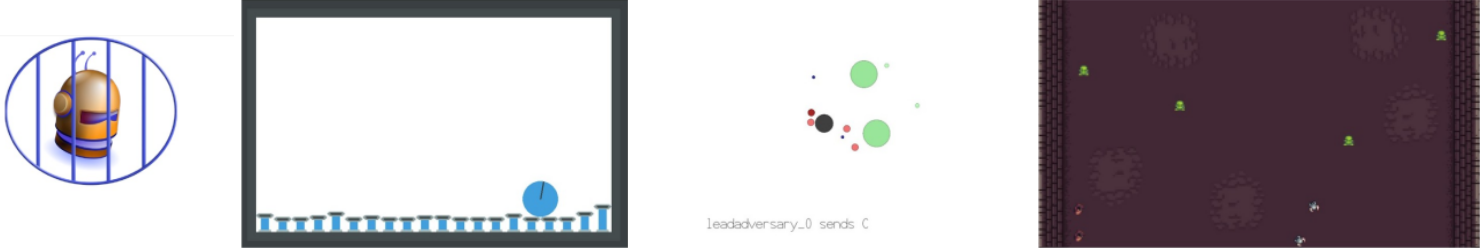
\includegraphics[width=0.8\linewidth]{figures/envs_4x1.png}
        \caption{Overview of the selected environments: CYB, PBL, PPY, and KAZ}
        \label{fig:simulated_environments}
    \end{figure}
    %
    \noindent We applied AOMEA in three cases:
    \begin{itemize}
        \item No organizational specifications (NTS): agents have to learn the most efficient collective strategies without any constraints or indications.
        \item Partially constraining organizational specifications (PTS): some constraints or indications are given to help converge faster or meet requirements.
        \item Fully constraining organizational specifications (FTS): manually crafted joint-policies are given for they are a reference regarding learned joint-policies.
    \end{itemize}

    \noindent Here, we do not present the details of the constraints that were given in NTS and FTS (available in Git repository\footnotemark[1]).
    %
    \begin{figure}[h!]
        \centering
        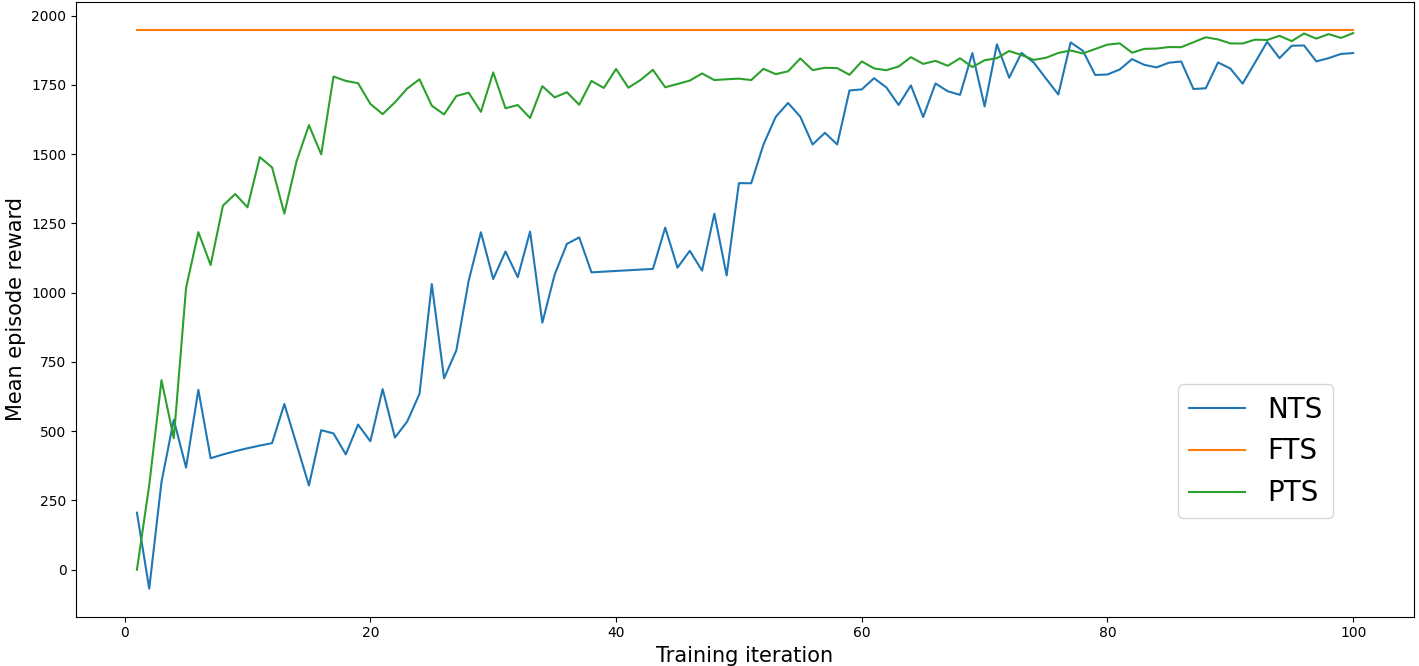
\includegraphics[width=0.8\textwidth]{figures/prahom_learning_curve.png}
        \caption{Average reward for each iteration in the PBL environment for the NTS, PTS, and FTS cases}
        \label{fig:prahom_learning_curve}
    \end{figure}
    %
    \begin{figure}[h!]
        \centering
        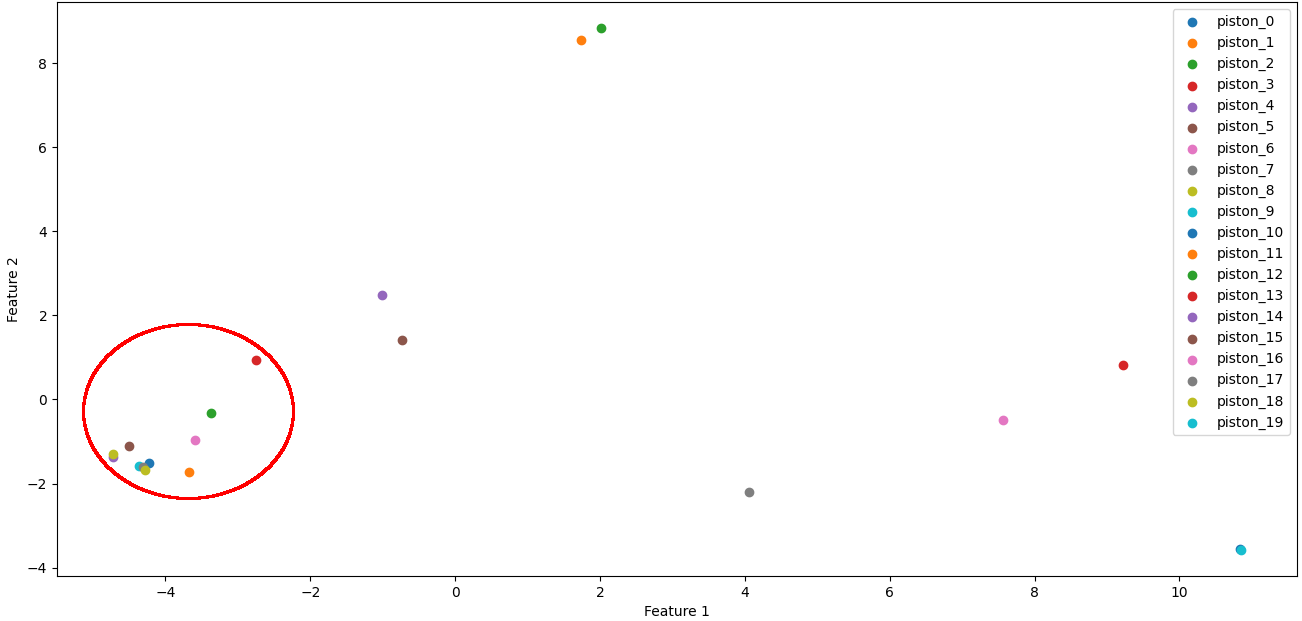
\includegraphics[width=0.8\textwidth]{figures/prahom_pca_analysis.png}
        \caption{PCA of the trained agents' histories in the PBL environment}
        \label{fig:prahom_pca_analysis}
    \end{figure}
    %
    We evaluate the impact of \emph{PRAHOM} on the following criteria: convergence time ratios between PTS, NTS, and FTS for reaching a threshold cumulative reward. Performance stability shows how the trained agents can achieve the goal generally by assessing several environments generated with different parameters. Results are presented in Table~\ref{tab:training_AOMEA_results}.
    %
    \begin{table}[t!]

    \centering

    \begin{tblr}{colspec={llll},rows={m},measure=vbox,stretch=-1}

        \textbf{Environment} & \textbf{PTS/NTS} & \textbf{PTS/FTS} & \textbf{Perf. stability \\ (avg. / max)} \\

        \hline

        { PPL }
        & { 4.7 }
        & { 1.3 }
        & { 0.9 } \\

        \hline[dashed]

        { PPY }
        & { 6.3 }
        & { 2.2 }
        & { 0.78 } \\

        \hline[dashed]

        { KAZ }
        & { 4.0 }
        & { 1.1 }
        & { 0.42 } \\

        \hline[dashed]

        { CYB }
        & { 12 }
        & { 3.3 }
        & { 0.36 } \\


    \end{tblr}

    \caption{View of the AOMEA approach impact during training}

    \label{tab:training_AOMEA_results}

\end{table}

    %
    As a general observation, we can notice convergence time is longer for NTS than for PTS which is also longer than for FTS. As expected, the search space is decreasing, hence a shorter convergence time. For instance, we noticed a faster convergence to a sub-optimal solution in the PBL environment by providing organizational specifications as presented in \autoref{fig:prahom_learning_curve}. Although PTS converges faster than NTS to a comparable cumulative reward, NTS may outperform PTS because trained agents' policies are hand-tailored to solve the problem much more finely than the designer's organizational specifications can do. Low-performance stability in the more complex CYB environment indicates that the trained agents have difficulty finding general strategies compared to the agents in the other environments.

    We also took into account the following criteria after training: roles, links, and global performance. A qualitative analysis is presented in Table~\ref{tab:trained_AOMEA_results}
    %
    \begin{table}[t!]

    \centering

    \begin{tblr}{colspec={llll},rows={m},measure=vbox,stretch=-1}

        \textbf{Environment} & \textbf{Roles} & \textbf{Links} & \textbf{Global performance} \\

        \hline

        { 1 }
        & {  }
        & {  } \\
        & {  } \\

        \hline[dashed]

        { 2 }
        & {  }
        & {  } \\
        & {  } \\

        \hline[dashed]

        { 3 }
        & {  }
        & {  } \\
        & {  } \\

        \hline[dashed]

        { 4 }
        & {  }
        & {  } \\
        & {  } \\

        \hline[dashed]

        { 5 }
        & {  }
        & {  } \\
        & {  } \\

    \end{tblr}

    \caption{View of the OOMARL approach impact after training}

    \label{tab:trained_OOMARL_results}

\end{table}

    %
    % //TODO: Moise+ schemes and comparison with expected ones
    %
    For the PBL environment, we can notice roles being equivalent for agents are expected to act the same. Indeed, trained agents' histories are close hence showing a common emerging role. We generate the PCA presented in \autoref{fig:prahom_pca_analysis} by expressing agents' histories as vectors containing the observation-action couples. We can notice most agents’ histories are in the left bottom zone (circled in red). It shows most pistons seem to act similarly as expected. We observe no organizational specifications except roles have been generated because agents cannot communicate. For the KAZ environment, we can notice two distinct roles: archers tend to move away from zombies, while knights tend to approach them. For the PPY environment, we can observe the output specifications indicate authority links between the leader predator and the simple predators to enable collective strategies for circling prey. Finally, the CYB environment shows communications between blue agents are indeed understood as communication links that enable isolating infiltrated drones or trying to fix and alert recently suspected drones.

    For the CYB environment, we developed our custom MAS via a simple hand-crafted decision tree as preconized in AOMEA in light of the organizational specifications we curated by removing noisy results. Our approach did not suggest general roles but relevant strategy patterns have been identified. For instance, regarding links between agents' roles, we noticed that the agents sending messages frequently seem to be spotted as suspected by their neighbors. In addition, a cyber-defender agent in the communication radius of a suspected drone tends to switch off its communication and reactivate afterward. Even though these insights are few, the mean score we got with our curated MAS is about -2000 which is indeed close to the top 5 scores. This shows AOMEA to be indeed applicable to the Cyberdefense context additionally bringing safety guarantees.


\end{frame}
